\documentclass[conference]{IEEEtran}
\IEEEoverridecommandlockouts
% The preceding line is only needed to identify funding in the first footnote. If that is unneeded, please comment it out.
\usepackage{cite}
\usepackage{amsmath,amssymb,amsfonts}
\usepackage{algorithmic}
\usepackage{graphicx}
\usepackage{textcomp}
\usepackage{xcolor}
\def\BibTeX{{\rm B\kern-.05em{\sc i\kern-.025em b}\kern-.08em
    T\kern-.1667em\lower.7ex\hbox{E}\kern-.125emX}}

%\usepackage{amsmath,amssymb,amsfonts}
%\usepackage{algorithmic}
%\usepackage{graphicx}
%\usepackage{textcomp}
%\usepackage{xcolor}


%\usepackage{cite}
\usepackage{booktabs}   %% For formal tables:
                        %% http://ctan.org/pkg/booktabs
\usepackage{subcaption} %% For complex figures with subfigures/subcaptions
                        %% http://ctan.org/pkg/subcaption
\usepackage{array}
%\usepackage{amsmath,amsfonts}
%\usepackage{algorithm}
%\usepackage[noend]{algpseudocode}
%\usepackage{algorithmic}
%\usepackage{graphicx}
%\usepackage{textcomp}
\usepackage{float}
\usepackage{listings}
\usepackage{xspace}
\usepackage{multirow}
\usepackage{amsthm}
\usepackage{enumitem}

\newtheorem{definition}{Definition}
\newtheorem{key-idea}{Key Idea}
\usepackage{balance}
\usepackage{printlen}
\usepackage[skins]{tcolorbox}

%\usepackage{xcolor,pifont}
%\newcommand*\colourcheck[1]{%
%	\expandafter\newcommand\csname #1check\endcsname{\textcolor{#1}{\ding{52}}}%
%}
%\colourcheck{blue}
%\colourcheck{green}
%\colourcheck{red}

\newtcolorbox{myframe}[2][]{%
  enhanced,colback=white,colframe=black,coltitle=black,
  sharp corners,
  toprule=1.0pt,
  rightrule=0.3pt,
  leftrule=0pt,
  bottomrule=0pt,
  fonttitle=\itshape\scshape\large,
  left=0pt,right=5pt,top=5pt,bottom=3pt,
  attach boxed title to top right={yshift=-0.3\baselineskip-0.4pt,xshift=-5mm},
  boxed title style={tile,size=minimal,left=0.2mm,right=0.5mm,
    colback=white,before upper=\strut},
  title=#2,#1
}

%\newcommand{\code}[1]{{\footnotesize\textsf{#1}}}

\newcommand{\checkNum}[1]{#1}

\newcommand{\tool}{\textsc{ABC}\xspace}

\newtheorem{Definition}{Definition}
\newtheorem{Claim}{Claim}
\newtheorem{Lemma}{Lemma}
\newtheorem{Theorem}{Theorem}

\newcolumntype{L}[1]{>{\raggedright\arraybackslash}p{#1}}
\newtheorem{Observation}{Observation}
\newtheorem{property}{Property}
\newcommand{\code}[1]{{\footnotesize\texttt{#1}}}
\usepackage{amsthm}
 \definecolor{dkgreen}{rgb}{0,0.6,0}
\definecolor{gray}{rgb}{0.5,0.5,0.5}
\definecolor{mauve}{rgb}{0.58,0,0.82}
\lstset{frame=tb,
  language=Java,
  aboveskip=3mm,
  belowskip=3mm,
  showstringspaces=false,
  columns=flexible,
  basicstyle={\small\ttfamily},
  numbers=left,
  numberstyle=\tiny\color{gray},
  keywordstyle=\color{blue},
  commentstyle=\color{dkgreen},
  stringstyle=\color{mauve},
  breaklines=true,
  breakatwhitespace=true,
  tabsize=4
}


%\usepackage{tikz}
%\usetikzlibrary{shapes.arrows}
%\newcommand{\FancyUpArrow}{\begin{tikzpicture}[baseline=-0.3em]
%		\node[single arrow,draw,rotate=90,single arrow head extend=0.1em,inner
%		ysep=0.1em,transform shape,line width=0.03em,top color=green,bottom color=green!50!black] (X){};
%\end{tikzpicture}}

%\def\BibTeX{{\rm B\kern-.05em{\sc i\kern-.025em b}\kern-.08em
%    T\kern-.1667em\lower.7ex\hbox{E}\kern-.125emX}}


\begin{document}

%\title{Conference Paper Title*\\
%{\footnotesize \textsuperscript{*}Note: Sub-titles are not captured in Xplore and
%should not be used}
%\thanks{Identify applicable funding agency here. If none, delete this.}
%}

%\makeatletter
%\newcommand{\linebreakand}{%
%\end{@IEEEauthorhalign}
%\hfill\mbox{}\par
%\mbox{}\hfill\begin{@IEEEauthorhalign}
%}
%\makeatother

\title{Title goes here}

%\author{\IEEEauthorblockN{Aashish Yadavally and Tien N. Nguyen}
%\IEEEauthorblockA{\textit{Computer Science Department} \\
%\textit{The University of Texas at Dallas}\\
%Texas, USA \\
%\{aashish.yadavally, tien.n.nguyen\}@utdallas.edu}
%\and
%\IEEEauthorblockN{Wenbo Wang and Shaohua Wang}
%\IEEEauthorblockA{\textit{Department of Informatics} \\
%\textit{New Jersey Institute of Technology}\\
%New Jersey, USA \\
%ww6@njit.edu, davidshwang@ieee.org}
%}

\maketitle

\begin{abstract}
Abstract goes here.
\end{abstract}

%\begin{IEEEkeywords}
%neural partial program analysis, neural program dependence analysis, neural networks; deep learning
%\end{IEEEkeywords}

\section{Introduction}
\label{sec:intro}

Software libraries provide an excellent mechanism for practical
software reuse. Each library provides its functionality through the
Application Programming Interfaces (APIs). The library's designers
have the intent for developers to use the APIs in specific
combinations and orders to achieve its functionality. Such correct API
usages are often described in {\em API specifications}. A common
phenomenon in programming with libraries is API misuses. API misuses
are the incorrect usages that violate the usage constraints of the
APIs involving in an API usage to achieve certain task.  For example,
to correctly use an \code{Iterator}, one must check that
\code{Iterator.hasNext()} returns \code{true} before calling
\code{Iterator.next()} on the \code{Iterator} object. Otherwise,
an \code{NoSuchElementException} will be thrown at run-time.

API misuses have been shown to cause several issues ranging from
run-time errors, program crashes, null-pointer exceptions, to security
vulnerabilities~\cite{mudetect-msr19,MM13,SHA15,FHMB+12,EBFK13,NKMB16,GIJA+12,ANNN+16}. To
mitigate API misuse, researchers have proposed several
\emph{API-misuse
detectors}~\cite{LZ05,L07,WZL07,RGJ07,NNP+09,AX09,TX09,TX09b,WZ11,MM13,NPVN16}.
These detectors analyze a given \emph{API usage}, i.e., a code snippet
that use a given API, and detect if it contains an API misuse.  In
general, the API misuse detection approaches can be broadly classified
into two categories. In the first category, the approaches mine the
API specifications from the API documentation and then check the code
against
them~\cite{ase22,jdoctor-issta18,zhou-icse17,c2s-fse20}. However,
these approaches are limited in two ways. First, the lack of
specifications in the API documentation in general has been hindering
the libraries' users in understanding and using the APIs in the
correct manner. The reason is that manually defining specifications is
time-consuming. The libraries' developers must spend additional time
and effort for documenting API specifications. Second, the existing
API specification mining approaches work only for specific types of
specifications, e.g., behavioral exceptions~\cite{ase22}, temporal
orders~\cite{icse17-nier}, etc. Moreover, they are limited due to
explicitly pre-defined rules for lexical and semantic matching of
texts to derive conditions from API
documentation~\cite{zhou-icse17,jdoctor-issta18}.

%Incorrect usages of an Application Programming Interface (API), or \emph{API misuses}, are violations of (implicit) \emph{usage constraints} of the API.
%An example of a usage constraint is having to check that \code{hasNext()} returns \code{true} before calling \code{next()} on an \code{Iterator}, in order to avoid a \code{NoSuchElementException} at runtime.
%API misuse is a prevalent cause of software bugs, crashes, and vulnerabilities~\cite{MM13,SHA15,FHMB+12,EBFK13,NKMB16,GIJA+12,ANNN+16}.

% While good API documentation might mitigate the problem, a recent study shows that Android developers, for example, prefer informal references, such as StackOverflow, over official API documentation, even though the former promote many insecure API usages~\cite{ABFKMS16}.
% Previous work also indicates that developers struggle with well-documented APIs, such as Java's \code{Iterator}~\cite{ANNN+17}.
% Therefore, in addition to improving documentation, techniques have been developed to detect misuses and warn developers about them.
%

The second category of API misuse detectors relies on {\em pattern
  mining}~\cite{LZ05,L07,WZL07,RGJ07,NNP+09,AX09,TX09,TX09b,WZ11,MM13,NPVN16}. First,
they mine from the large code corpus the {\em API usage patterns},
which are the API usages occurring frequently. These mined API usage
patterns are considered as the correct ones. The given code is then
processed to check for any deviations from these patterns.  If true,
it is considered as a potential API misuse. Unfortunately, the
reported precision of such detectors is typically low and a recent
study~\cite{ANNN+17} showed that their recall is also very low.
%Tien: key issue
The still-prevalent problems of API misuse detectors have been
reported~\cite{LHXRM16,ABFKMS16}. First, the mining-based detectors
cannot differentiate infrequent from invalid usage. This is an
inherent issue with mining because these approaches need to set a
pre-defined threshold for frequent API usage patterns. This also leads
to the second problem: the detectors often learn a pattern and then
report instances of alternative usages as violations. Alternative
usage is a different functionally correct way to use an API to achieve
the same functionality.


%%%
%%%Previous work identified individual as well as common strengths and weaknesses of existing detectors~\cite{ANNN+17} in an empirical study using the open-source benchmark MUBench~\cite{mubench}.
%%%In this paper, we investigate whether addressing the reported weaknesses indeed leads to better performance in practice.
%%%% representation
%%%Therefore, we design a new misuse detector, MUDetect.
%%%MUDetect encodes API usages as API-Usage Graphs, a comprehensive usage representation that captures different types of API misuses.
%%%% domain knowledge
%%%MUDetect employs a greedy, frequent-subgraph-mining algorithm to mine patterns and a specialized graph-matching strategy to identify pattern violations. % (violating) pattern occurrences.
%%%Both components consider code semantics to improve the overall detection capabilities.
%%%% ranking
%%%On top, MUDetect uses an empirically optimized ranking strategy to effectively rank true positives.
%%%While previous detectors mostly target a per-project setting~\cite{ANNN+17}, MUDetect also works in a cross-project setting, where it mines thousands of usage examples from third-party projects.
%%%
%%%% evaluation
%%%We assess the precision and recall of MUDetect and show that it outperforms the \checkNum{four} state-of-the-art detectors evaluated in prior work~\cite{ANNN+17}.
%%%% dataset
%%%In our evaluation, we extended MUBench by \checkNum{107} real-world misuses identified in a recent study on run-time verification~\cite{LHXRM16}---\checkNum{more than doubling} its size---to ensure that our design decisions generalize.
%%%%
%%%%results
%%%% intra project
%%%We show that, in a setting with perfect training data, MUDetect achieves a recall of \checkNum{72.5\%}, which is \checkNum{20.3\%} higher than the next best detector and over \checkNum{50\%} higher than the other detectors.
%%%In the typical per-project setting, MUDetect achieves recall of \checkNum{20.9\%}, which is \checkNum{10.2\%} better than the second-best detector, and precision of \checkNum{21.9\%}, which is \checkNum{13.1\%} better than the second-best detector.
%%%% cross project
%%%In a cross-project setting, MUDetect's recall and precision again improve significantly to \checkNum{42.2\%} and \checkNum{33.0\%}, respectively.
%%%%
%%%% pull requests
%%%Throughout the experiments, MUDetect identified 27 previously unknown misuses, which we reported in \checkNum{eight} pull requests (PRs).
%%%To date, \checkNum{three} of the PRs got accepted, demonstrating that MUDetect identifies actual issues in current software projects.


%%%To summarize, this paper makes the following contributions:
%%%%
%%%\begin{itemize}[leftmargin=*]
%%%  \item AUG, a graph-based representation of API usages that captures all usage properties relevant for identifying misuses.
%%%  \item Code-semantic-aware, greedy frequent-subgraph-mining and graph-matching algorithms to identify patterns within and across projects and (violating) instances in a target codebase.
%%%  \item MUDetect, a (cross-project) misuse detector.
%%%  \item An empirical study of ranking strategies to improve precision.
%%%  \item An empirical evaluation that compares MUDetect to existing detectors, and includes an analysis of the results to identify further opportunities for improvement.
%%%  \item Fixes for all previously unknown misuses identified by MUDetect, for external validation of the findings' relevance.
%%%\end{itemize}
%%%
%%%We publish our MUBench extension, MUDetect's implementation, and all experiment data, tooling, and results~\cite{artifact-page}.

In this paper, we address those above problems with the mining-based
API misuse detection approaches. We introduce {\tool}, a
learning-based API misuse detection approach, that leverages two key
insights to overcome those issues. First, we use a graph
representation, called Augmented Usage Graph
(AUG)~\cite{mutetect-msr19}, to represent the program dependencies and
relations among the API elements as well as other program elements in
an API usage. We then use the Graph Convolutional Network (GCN) to
model the API usage by encoding the corresponding AUG. Second, due to
the lack of training data for the code with API misuses, we apply
several techniques for data augmentation.


%We extract the AUGs from the complete, compilable source code using
%the APIs from a large code corpus. We then enhance the AUGs with all
%the FQNs because the training code is compilable.


\section{Motivating Examples}
\label{sec:motiv}

\subsection{Examples}

\begin{figure}[t]
	\centering
	\lstset{
		numbers=left,
		numberstyle= \tiny,
		keywordstyle= \color{blue!70},
		commentstyle= \color{red!50!green!50!blue!50},
		frame=shadowbox,
		rulesepcolor= \color{red!20!green!20!blue!20} ,
		xleftmargin=1.5em,xrightmargin=0em, aboveskip=1em,
		framexleftmargin=1.3em,
                numbersep= 3pt,
%                numbersep=-12pt,
                framexrightmargin=-3mm,
		language=Java,
                basicstyle=\scriptsize\ttfamily,
                numberstyle=\scriptsize\ttfamily,
                emphstyle=\bfseries,
                moredelim=**[is][\color{red}]{@}{@},
		escapeinside= {(*@}{@*)}
	}
\begin{lstlisting}[]
class HttpMethodDirector {
  AuthState authstate = method.(*@{\color{red}{getHostAuthState}@*)();
  if (authstate.(*@{\color{red}{isPreemptive}@*)()) {
    authstate.(*@{\color{red}{invalidate}@*)();
(*@{\color{cyan}{\quad + authstate.}@*)(*@{\color{red}{setAuthRequested(true);}@*)
  }
  Map challenges = AuthChallengeParser.parseChallenges(
  method.getResponseHeaders(WWW_AUTH_CHALLENGE));
  ...
\end{lstlisting}
        \vspace{-12pt}
        \caption{An API misuse in Apache \code{HttpClient} project}
        \vspace{-6pt}
        \label{fig:example1}
\end{figure}

Let us use real-world examples to illustrate the problem and motivate
our solution. Fig.~\ref{fig:example1} displays an API misuse in
MuBench~\cite{mudetect-msr19}, an API misuse dataset. The code shows
the usage of the API elements in \code{httpclient} of Apache.  The
intended usage of the API elements is that when
\code{Auth\-State.\-is\-Pre\-emptive\-()} returns true (i.e., the
status of the current authentication is preemptive), both
\code{Auth\-State.\-invalidate()} and
\code{Auth\-State.\-set\-Auth\-Requested(true)} must be called. The
purpose is to invalidate the current request and to set the need for
an authentication for a later operation. However, the latter call was
missing. Thus, line 5 was added to fix the~misuse.

\begin{figure}[t]
	\centering
	\lstset{
		numbers=left,
		numberstyle= \tiny,
		keywordstyle= \color{blue!70},
		commentstyle= \color{red!50!green!50!blue!50},
		frame=shadowbox,
		rulesepcolor= \color{red!20!green!20!blue!20} ,
		xleftmargin=1.5em,xrightmargin=0em, aboveskip=1em,
		framexleftmargin=1.3em,
                numbersep= 3pt,
%                numbersep=-12pt,
                framexrightmargin=-3mm,
		language=Java,
                basicstyle=\scriptsize\ttfamily,
                numberstyle=\scriptsize\ttfamily,
                emphstyle=\bfseries,
                moredelim=**[is][\color{red}]{@}{@},
		escapeinside= {(*@}{@*)}
	}
\begin{lstlisting}[]
private void authenticateHost(final HttpMethod method) {
  ...
  if (LOG.isWarnEnabled()) {
    LOG.warn(``Required credentials not available'');
    if (method.(*@{\color{red}{getHostAuthState().isPreemptive()}@*)) {
      LOG.warn(``Preemptive authentication requested but no default credentials available'');
      method.getHostAuthState().(*@{\color{red}{invalidate();}@*)
      method.getHostAuthState().(*@{\color{red}{setAuthRequested(true);}@*)
  }
}
\end{lstlisting}
        \vspace{-12pt}
        \caption{Gihub project \code{jerenkrantz}}
        \vspace{-6pt}
        \label{fig:example2}
\end{figure}

This usage scenario is one of the intended usages of the
\code{httpClient} library. As a result, the API usage repeats in other
projects. Fig.~\ref{fig:example2} shows the same usage in the Github
project \code{jerenkrantz}. Despite the differences in the details of
surrounding code, the sequence/orders of the relevant API elements
\code{getHostAuthState}, \code{isPreemptive}, \code{invalidate}, and
\code{setAuthRequested} are the same.

%\vspace{2pt}
%\noindent {\bf Observation 1} [{\em Regularity of API Usages}]. The
%designers of software libraries have the intents for developers to use
%the API elements together (including API classes, method calls, field
%accesses) in certain combinations/orders to achieve a programming
%task.

\begin{Observation}[Regularity of API usages]
The designers of software libraries have the intention for the API
elements to be used together (including API classes, method calls,
field accesses) in certain combinations/orders to achieve a
programming task.
\end{Observation}

This observation motivates a learning-based approach that could
leverage the regularity of API usages without the need of a threshold
as in the mining-based approaches. A machine learning (ML) model could
learn the API usages from existing code corpus to decide whether the
current API usage conforms or violates API usage specifications.

Compared the usages in Fig.~\ref{fig:example1} and
Fig.~\ref{fig:example2}, we can see that the surrounding code contexts
of the above relevant API elements can be different and are less
important in deciding whether the current API usage is a violation or
not. For example, the lines 7--8 in Fig.~\ref{fig:example1} for
handling response headers and lines 3,4, and 6 in
Fig.~\ref{fig:example2} to deal with logging are less crucial than the
lines with \code{getHostAuthState}, \code{isPreemptive},
\code{invalidate}, and \code{setAuthRequested}.

\begin{Observation}[API elements in API usages]
To decide an API misuse, one needs to examine the API elements
including API classes, method calls, field accesses together with the
data and control dependencies among them and other relevant program
elements.
\end{Observation}

%\subsection{Key Ideas}
\label{sec:key-ideas}

From the above observations, we draw the following key ideas for our
approach.

\begin{key-idea}[Deep Learning for API usages]
We leverage Machine Learning to implicitly learn co-occurring API
elements in API usages. From the basis of the regularity of API
usages: the API elements regularly appearing together in API usages
have higher impact in establishing the correct API usages than the
less regular ones. Importantly, the learning-based direction helps
avoid the use of thresholds in either establishing the API usage
patterns or distinguishing between the misuses and the uncommon
usages, as in the mining-based API misuse detection approaches. We
could leverage the complete, compilable code using the libraries from
a large code corpus, in which all the API elements in use are known.
\end{key-idea}


\begin{key-idea}[Data Augmentation for API Usages and Misuses]
...
\end{key-idea}

\begin{key-idea}[Graph-based Neural Network Model for API Usages]
...
\end{key-idea}





\subsection{Key Ideas}
\label{sec:key-ideas}

From the above observations, we draw the following key ideas for our
approach.

\begin{key-idea}[Deep Learning for API usages]
We leverage Machine Learning to implicitly learn co-occurring API
elements in API usages. From the basis of the regularity of API
usages: the API elements regularly appearing together in API usages
have higher impact in establishing the correct API usages than the
less regular ones. Importantly, the learning-based direction helps
avoid the use of thresholds in either establishing the API usage
patterns or distinguishing between the misuses and the uncommon
usages, as in the mining-based API misuse detection approaches. We
could leverage the complete, compilable code using the libraries from
a large code corpus, in which all the API elements in use are known.
\end{key-idea}


\begin{key-idea}[Data Augmentation for API Usages and Misuses]
...
\end{key-idea}

\begin{key-idea}[Graph-based Neural Network Model for API Usages]
...
\end{key-idea}




\section{Important Concepts}
\label{sec:concepts}

This section describes the definitions of the important concepts
regarding our representations on API usages.

%\begin{figure}[t] %[!htp]
%	\centering
%	\includegraphics[width=0.9\linewidth]{aug-example}
%        \vspace{-3pt}
%	\caption{An API Usage and its API-Usage Graph}
%	\label{fig:aug}
%\end{figure}

\begin{Definition}[API elements]
An API element is either a class, a method, or a field that is
provided in a library to enable the accesses to the library's
functions via a variable declaration with a certain class, a method
call to an API method, or a field access to an API field.
\end{Definition}

For example, in Fig.~\ref{fig:example1}, line 2, \code{AuthState} is
an API class, which is a declared type for the variable
\code{authstate}. At line 3, \code{isPreemptive} is an API
method, which is called on the variable \code{authstate}.

\begin{Definition}[API Usage]
An API usage consists of a set of API elements and control structures
(i.e., conditions and repetitions), together with other program
elements (e.g., variables, parameters, etc.) in specific combinations
and orders to perform a programming task.
\end{Definition}

In Fig.~\ref{fig:example1}, lines 2-5 show an API usage consisting of
1) a variable \code{authstate}, 2) its declared class
\code{AuthState}, 3) a method call to \code{getHostAuthState()} on the
variable \code{method}, 4) a method call to \code{isPreemptive()}, 5)
a conditional structure with \code{if}, 6) a method call to
\code{invalidate()}, and 6) a method call to
\code{setAuthRequested(...)}.

To represent an API usage, we adopt a graph-based representation
called {\em API-Usage Graphs (AUGs)}~\cite{msr19}.

\begin{Definition}[API Usage Graph (AUG)~\cite{msr19}]
AUG is a directed, connected graph with labelled nodes and
edges. Nodes represent data entities (variables, values), and actions,
(method calls or operators). Edges represent the API usage
relations among the entities and actions represented by nodes.
\end{Definition}

The usage relations are defined as follows.

\begin{Definition}[API Usage Relation]
  In an API usage, there exist the API usage relations among the API
  elements and relevant program elements. The API usage relations
  include the following ones: {\bf receiver, parameter, definition,
    order, condition, synchronize, throw, handle}, and {\bf data and
    control dependencies} among the API and program elements.
\end{Definition}

Let us use the term {\em action nodes} to refer to method calls, field
accesses, or operators, and the term {\em data nodes} to represent
objects, values, and literals that appear in API usages. A {\em
  receiver} relation exists between a variable and a method call. In
Fig.~\ref{fig:example2}, at line 3, there exists a receiver relation
between the variable \code{myButton} and the method
\code{addClickHandler}. A {\em parameter} relation connects an
argument to be used as a parameter of an action. A {\em definition}
relation exists between a constructor or method call that creates or
returns a value or object to the respective variable. An {\em order}
relation connects two actions on operating on the same receiver or
parameter. A {\em condition} relation connects an action whose result
controls branching to an action being controlled. A {\em synchronize}
relation connects a variable that the program obtains a lock on to an
action executed under that lock. A {\em throw} relation connects an
action that may throw an exception to a data node representing that
exception object. A {\em handle} relation connects from a \code{catch}
action to an action in a respective exception handling block.

We expect to leverage those API usage relations among the API elements
and relevant program entities to learn the FQNs.



%Fig.~\ref{fig:aug} shows an example of an API usage and its AUG.
%The action nodes are displayed in the rectangles and the data nodes in
%the oval shapes. The action nodes represent constructor calls
%(\code{init}), method calls, field accesses, and operators. If the
%types are available, they will be resolved. However, in the figure,
%only the simple name is shown for clarity. The relational operators
%are also encoded as actions to capture conditions. The data nodes
%represent objects, values, and literals in an API usage. AUG encodes
%data entities as nodes to make explicit the data dependencies between
%actions, such as multiple calls on the same object to ensure we have a
%connected subgraph with all data-dependent parts of a usage. The usage
%relations are shown with their labels. {\em Order} edges are not
%shown for clarity. The AUG building algorithm is explained in~\cite{msr19}.


\section{Data Augmentation for API usages}
\label{sec:data-aug}




\section{Architecture Overview}
\label{sec:overview}

\begin{figure*}[t]
\begin{center}
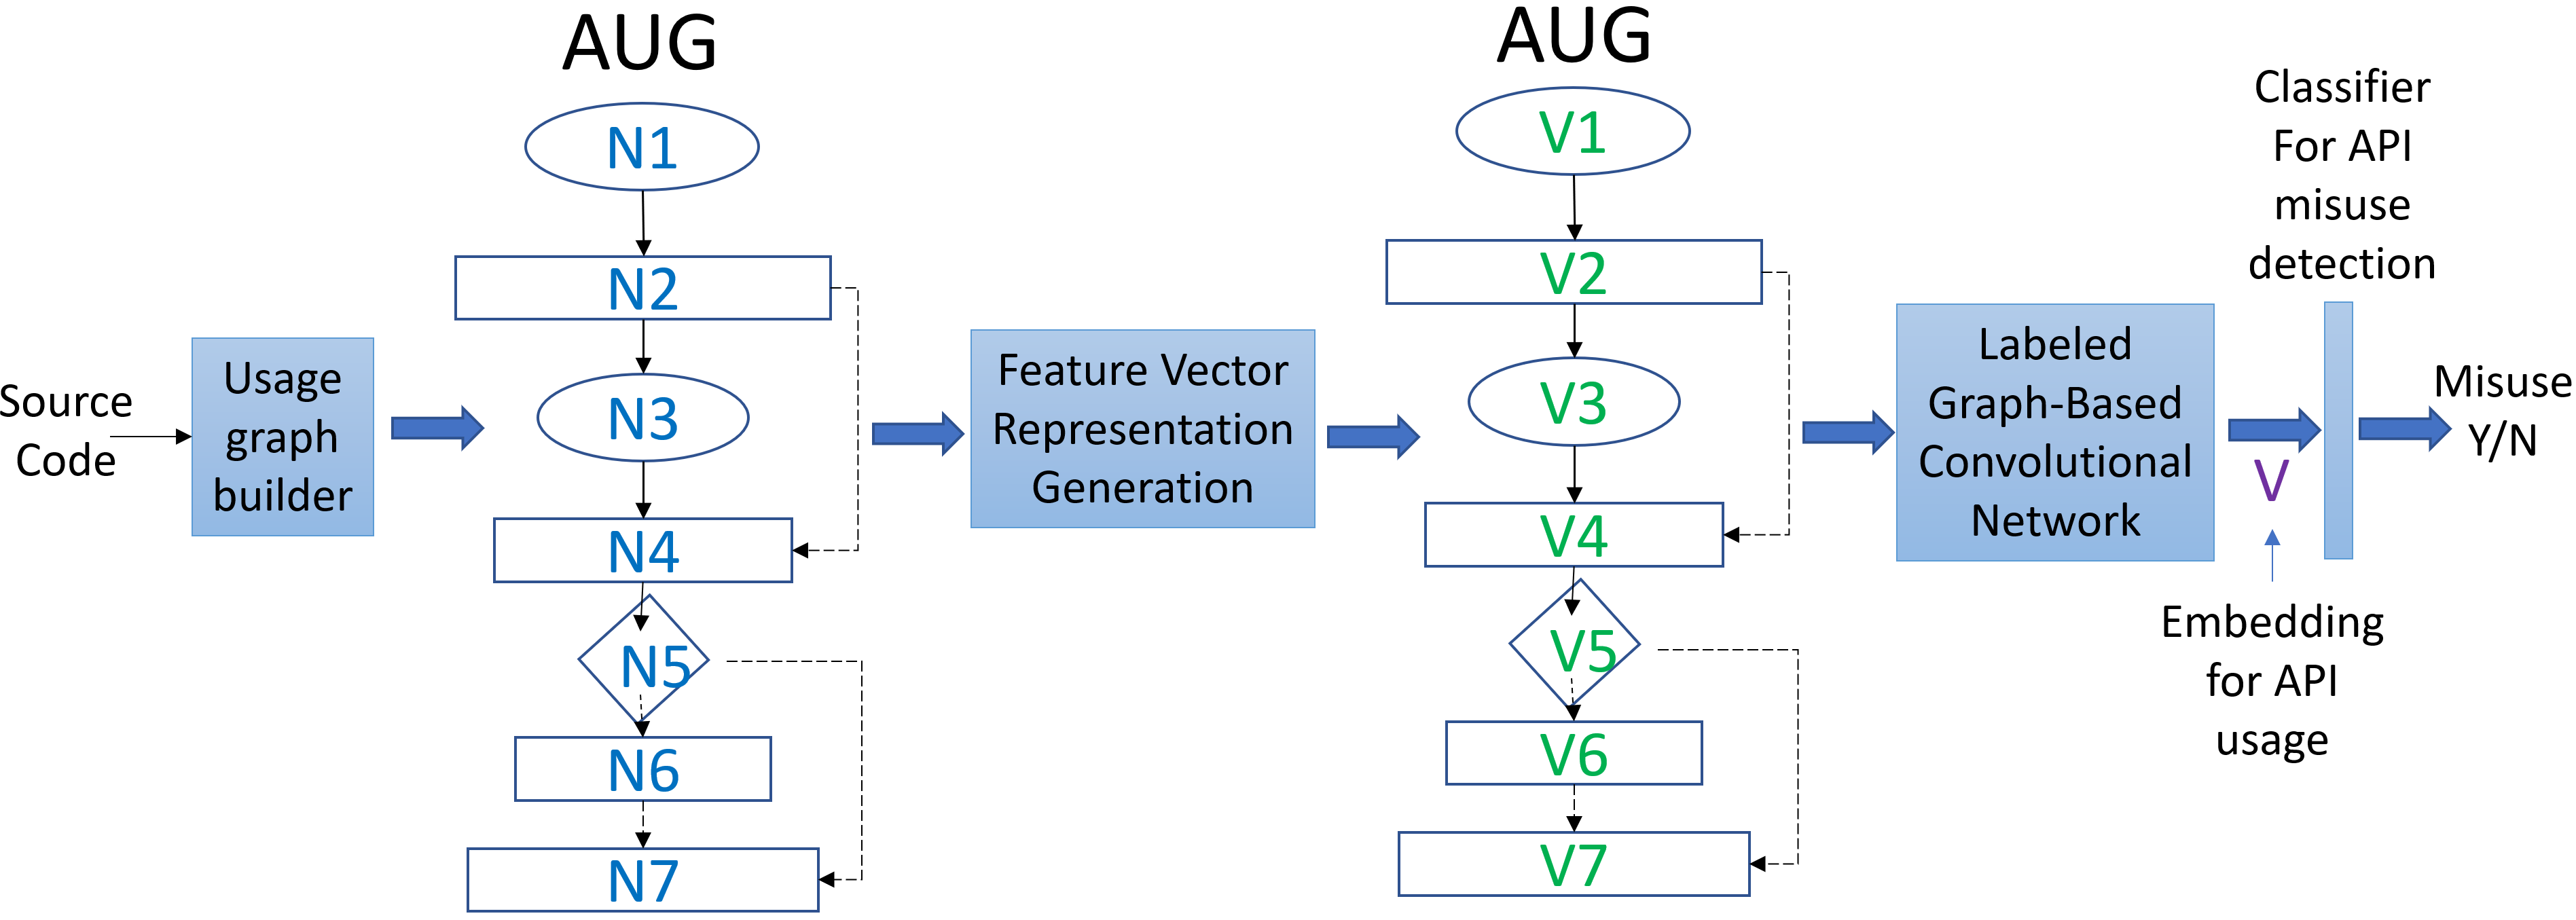
\includegraphics[width=5.4in]{overview.png}
\vspace{-5pt}
\caption{{\tool}: Architecture Overview}
\label{overview}
\end{center}
\end{figure*}

In general, {\tool} has three main components. 


\subsection{Code Feature Representation Learning}
\label{sec:features}

An API element at a node in the AUG built from a method is represented
via a sequence of the sub-tokens extracted from the node's
content. The sub-token granularity for source code has been shown to
have higher regularity than tokens~\cite{icse20-methodname}. Each name
of an API element at a node is tokenized using CamelCase or Hungarian
convention. Only variables, methods, fields, and class' names
are kept. The sub-tokens with one character are removed to avoid
noises. We then treat each sequence of sub-tokens as a sentence and
use a word embedding technique~\cite{glove2014} to build the vectors
for the sub-tokens.  The vector for the sequence of sub-tokens is used
for the node.


%\input{eval}

%\input{empirical-results}

%\input{related-work}

%\section*{Acknowledgments}
%This work was supported in part by the US National Science Foundation
%(NSF) grants CNS-2120386.

%\newpage

%\balance

\bibliographystyle{IEEEtran}

\bibliography{references,ase22,tien}

\end{document}
